\documentclass[11pt,authoryear]{article}
\pdfoutput = 1
\usepackage{fullpage,amsthm,amsmath,natbib,algorithm,algorithmic,enumitem,afterpage,amssymb,setspace,graphicx,amsfonts,array,verbatim,commath,mathrsfs}
\usepackage[dvipsnames]{xcolor}
\usepackage{tikz}
\usetikzlibrary{arrows,matrix,positioning, fit, shapes.geometric}
\usepackage[hang,flushmargin]{footmisc}
\usepackage[colorlinks=TRUE,citecolor=Blue,linkcolor=BrickRed,urlcolor=PineGreen]{hyperref}
\newtheorem{lemma}{Lemma}
\newtheorem{theorem}{Theorem}
\newtheorem{proposition}{Proposition}
\newtheorem{corollary}{Corollary}
\newtheorem{claim}{Claim}
\newtheorem{definition}{Definition}
\newtheorem{exmp}{Example}[section]
\allowdisplaybreaks
\renewcommand{\baselinestretch}{1.5}
\DeclareMathOperator*{\diag}{diag}
\DeclareMathOperator*{\cov}{cov}
\DeclareMathOperator*{\rank}{rank}
\DeclareMathOperator*{\var}{var}
\DeclareMathOperator*{\tr}{tr}
\DeclareMathOperator*{\veco}{vec}
\DeclareMathOperator*{\uniform}{\mathcal{U}niform}
\DeclareMathOperator*{\argmin}{arg\ min}
\DeclareMathOperator*{\argmax}{arg\ max}
\DeclareMathOperator*{\N}{N}
\DeclareMathOperator*{\gm}{Gamma}
\bibliographystyle{plainnat}
\newcommand*{\doi}[1]{\href{http://dx.doi.org/#1}{doi: #1}}
\newcommand{\bs}[1]{\boldsymbol{#1}}

\begin{document}
\singlespacing
\title{Derivation of VEM for M\&MASH}
\author{David Gerard}
\maketitle

\begin{abstract}
  Here, I derive the VEM algorithm for M\&MASH. This is not for final
  publication, but only for my own notes.
\end{abstract}

\section{Setup}
\label{section:setup}

I now describe the notation used in this text. I denote matrices by
boldface uppercase letters ($\bs{A}$), vectors are denoted by boldface
lowercase letters ($\bs{a}$), and scalars are denoted by non-boldface
letters ($a$ or $A$). All vectors are column-vectors. Lowercase
letters may represent elements of a vector or matrix if they have
subscripts. For example, $a_{ij}$ is the $(i,j)$th element of
$\bs{A}$, $a_i$ is the $i$th element of $\bs{a}$, and $\bs{a}_{i}$ is
either the $i$th row or $i$th column of $\bs{A}$. For indexing, we
will generally use capital non-boldface letters to denote the total
number of elements and their lowercase non-boldface versions to denote
the index. For example, $i = 1,\ldots,I$. We let $\bs{A}_{n \times p}$
denote that $\bs{A} \in \mathbb{R}^{n \times p}$. We denote the matrix
transpose by $\bs{A}^\intercal$, the matrix inverse by $\bs{A}^{-1}$,
and the matrix determinant by $\det(\bs{A})$. Finally, sets will be
denoted by calligraphic letters ($\mathcal{A}$).

We assume the following model
\begin{align}
\bs{Y}_{N\times M} = \bs{X}_{N \times K}\bs{B}_{K \times M} + \bs{Z}_{N \times R}\bs{A}_{R \times M} + \bs{E}_{N \times M},
\end{align}
where
\begin{align}
\bs{E} &\sim \N_{N \times M}(\bs{0}, \bs{\Lambda}^{-1} \otimes \bs{I}_N),\\
\bs{\Lambda} &= \diag(\lambda_1,\ldots,\lambda_M),\\
\bs{Z} &\sim \N_{N\times R}(\bs{0}, \bs{I}_R \otimes \bs{I}_N).
\end{align}
That is, the overall covariance of the columns of $\bs{Y}$ is
$\bs{A}^{\intercal} \bs{A} + \bs{\Lambda}$, a diagonal plus low rank
matrix. We place iid mixtures of normals prior on the rows of $\bs{B}$
and gamma priors on $\bs{\Lambda}$.
\begin{align}
\lambda_m &\overset{iid}{\sim} \gm(\alpha, \beta),\\
\bs{B} &=
\left(
\begin{array}{c}
\bs{b}_1^\intercal\\
\vdots\\
\bs{b}_K^\intercal\\
\end{array}
\right),\\
\bs{b}_k &\text{ i.i.d. s.t. } p(\bs{b}_k) = \sum_{t = 0}^T\pi_t\N_M(\bs{b}_k | \bs{0}, \bs{V}_t),
\end{align}
where the $\bs{V}_t$'s are $m \times m$ known positive semi-definite
covariance matrices and the $\pi_t$'s are proportions to be
estimated. We augment the prior of $\bs{b}_k$ by including a 1-of-$T$
indicator vector $\bs{w}_k \in \mathbb{R}^{T}$ denoting memborship of
$\bs{b}_k$ into one of the $T$ mixture groups and write
\begin{align}
p(\bs{b}_k|\bs{w}_k) &= \prod_{t = 0}^T\left[\N(\bs{b}_k|\bs{0},\bs{V}_t)\right]^{w_{kt}},\\
p(\bs{w}_k|\bs{\pi}) &= \prod_{t = 0}^T \pi_t^{w_{kt}}.
\end{align}
We could also place a normal prior on $\bs{A}$, but we
will instead also estimate it by ML.

The densities of all elements involved are
\begin{align}
\label{equation:Y.conditional}p(\bs{Y}|\bs{B}, \bs{Z}, \bs{A}, \bs{\Lambda}) &= (2\pi)^{-NM/2} \prod_{m = 1}^M \lambda_m^{N/2} \exp\left\{-\frac{1}{2}\tr\left[(\bs{Y}-\bs{X}\bs{B}-\bs{Z}\bs{A})\bs{\Lambda}(\bs{Y}-\bs{X}\bs{B} - \bs{Z}\bs{A})^{\intercal}\right]\right\}\\
p(\bs{Z}) &= (2\pi)^{-NR/2}\exp\left\{-\frac{1}{2}\tr[\bs{Z}\bs{Z}^{\intercal}]\right\}  \\
p(\lambda_m|\alpha,\beta) &= \frac{\beta^{\alpha}}{\Gamma(\alpha)}\lambda_m^{\alpha - 1}\exp\{-\beta\lambda_m\}\\
p(\bs{b}_k|\bs{w}_k) &= \sum_{t = 0}^{T}\left[(2\pi)^{-M/2}\det(\bs{V}_t)^{-1/2}\exp\left\{-\frac{1}{2}\bs{b}_k^{\intercal}\bs{V}_t^{-1}\bs{b}_k\right\}\right]^{w_{kt}}\\
\label{equation:w.conditional}p(\bs{w}_k|\bs{\pi}) &= \prod_{t = 0}^{T} \pi_t^{w_{kt}}.
\end{align}

\section{VEM}
Let $q$ be a function. The goal is to maximize over $(q, \bs{\pi},
\bs{A})$ the following lower-bound of the $\log$-marginal likelihood:
\begin{align}
\log p(\bs{Y}|\bs{\pi},\bs{A}) \geq \mathcal{L}(q, \bs{\pi}, \bs{A}) = \int q(\bs{B}, \bs{W}, \bs{Z}, \bs{\Lambda}) \log\left\{\frac{p(\bs{Y},\bs{B},\bs{W},\bs{Z},\bs{\Lambda}|\bs{\pi},\bs{A})}{q(\bs{B}, \bs{W}, \bs{Z}, \bs{\Lambda})}\right\}\dif\bs{B}\dif\bs{W}\dif\bs{Z}\dif\bs{\Lambda},
\end{align}
where
\begin{align}
p(\bs{Y},\bs{B},\bs{W},\bs{Z},\bs{\Lambda}|\bs{\pi},\bs{A}) = p(\bs{Y}|\bs{B}, \bs{Z}, \bs{A}, \bs{\Lambda})p(\bs{B}|\bs{W})p(\bs{W}|\bs{\pi})p(\bs{Z})p(\bs{\Lambda}),
\end{align}
where these densities are defined in equations \eqref{equation:Y.conditional} to \eqref{equation:w.conditional}.
We constrain $q$ to take the following form
\begin{align}
q(\bs{B}, \bs{W}, \bs{Z}, \bs{\Lambda}) = q(\bs{Z})q(\bs{\Lambda})\prod_{k = 1}^{K}q(\bs{b}_k,\bs{w}_k),
\end{align}
and thus perform mean-field variational inference.

\subsection{Update for $q(\bs{b}_k,\bs{w}_k)$}
By a general result in mean-field variational inference, we have
\begin{align}
\label{equation:general.bk}\log q(\bs{b}_k,\bs{w}_k)\propto E_{-(\bs{b}_k,\bs{w}_k)}\left\{\log p(\bs{Y},\bs{B},\bs{W},\bs{Z},\bs{\Lambda}|\bs{\pi},\bs{A})\right\},
\end{align}
where $E_{-(\bs{b}_k,\bs{w}_k)}[\cdot]$ is notation for the
expectation with respect to the $q$ distributions over all variables
except $\bs{b}_k$ and $\bs{w}_k$. See (10.9) of
\citet{bishop2006pattern}, for example. Here, I let ``$\propto$''
denote equality to up to an additive constant that is independent of
$\bs{b}_k$ and $\bs{w}_k$. So
\begin{align}
  \eqref{equation:general.bk} &\propto E_{-(\bs{b}_k,\bs{w}_k)}\left\{\log p(\bs{Y}|\bs{B}, \bs{Z}, \bs{A}, \bs{\Lambda}) + \log p(\bs{B}|\bs{W}) + \log p(\bs{W}|\bs{\pi})\right\}\\
  \begin{split}
    \label{equation:plugin.density}
    &\propto E_{-(\bs{b}_k,\bs{w}_k)}\left\{-\frac{1}{2}\tr\left[(\bs{Y}-\bs{X}\bs{B}-\bs{Z}\bs{A})\bs{\Lambda}(\bs{Y}-\bs{X}\bs{B} - \bs{Z}\bs{A})^{\intercal}\right]\right.\\
    & \left.+ \sum_{t = 0}^Tw_{kt}\left[-\frac{M}{2}\log(2\pi) - \frac{1}{2}\log\det(\bs{V}_t) - \frac{1}{2}\bs{b}_k^{\intercal}\bs{V}_t^{-1}\bs{b}_k + \log(\pi_t)\right]\right\}
  \end{split}
\end{align}
We note that
\begin{align}
\bs{X}\bs{B} = \sum_{\ell = 1}^K\bs{x}_{\ell}\bs{b}_{\ell}^{\intercal},
\end{align}
where $\bs{x}_k$ is the $k$th column of $\bs{X}$ and $\bs{b}_k$ is the $k$th row of $\bs{B}$. So
\begin{align}
\bs{Y} - \bs{Z}\bs{A} - \bs{X}\bs{B} = \bs{Y} - \bs{Z}\bs{A} - \sum_{\ell \neq k}\bs{x}_{\ell}\bs{b}_{\ell}^{\intercal} - \bs{x}_{k}\bs{b}_{k}^{\intercal}.
\end{align}
Let
\begin{align}
\bs{R}_{-k} := \bs{Y} - \bs{Z}\bs{A} - \sum_{\ell \neq k}\bs{x}_{\ell}\bs{b}_{\ell}^{\intercal},
\end{align}
then
\begin{align}
&\tr\left[(\bs{Y}-\bs{X}\bs{B}-\bs{Z}\bs{A})\bs{\Lambda}(\bs{Y}-\bs{X}\bs{B} - \bs{Z}\bs{A})^{\intercal}\right] = \tr\left[(\bs{R}_{-k} - \bs{x}_{k}\bs{b}_{k}^{\intercal})\bs{\Lambda}(\bs{R}_{-k} - \bs{x}_{k}\bs{b}_{k}^{\intercal})^{\intercal}\right]\\
&\propto \tr\left[\bs{x}_k\bs{b}_k^{\intercal}\bs{\Lambda}\bs{b}_k\bs{x}_k^{\intercal}\right] - 2\tr\left[\bs{x}_k\bs{b}_k^{\intercal}\bs{\Lambda}\bs{R}_{-k}^{\intercal}\right]\\
\label{equation:expand.bk}&= \|\bs{x}_k\|^2\bs{b}_k^{\intercal}\bs{\Lambda}\bs{b}_k -2\bs{b}_k^{\intercal}\bs{\Lambda}\bs{R}_{-k}^{\intercal}\bs{x}_k
\end{align}
Hence,
\begin{align}
  \begin{split}
    \eqref{equation:plugin.density} &\propto -\frac{1}{2}\left[\|\bs{x}_k\|^2\bs{b}_k^{\intercal}E\left[\bs{\Lambda}\right]\bs{b}_k - 2\bs{b}_k^{\intercal}E\left[\bs{\Lambda}\right]E\left[\bs{R}_{-k}\right]^{\intercal}\bs{x}_k\right]\\
    &+\sum_{t = 0}^Tw_{kt}\left[-\frac{M}{2}\log(2\pi) - \frac{1}{2}\log\det(\bs{V}_t) - \frac{1}{2}\bs{b}_k^{\intercal}\bs{V}_t^{-1}\bs{b}_k + \log(\pi_t)\right]
  \end{split}\\
  \begin{split}
    \label{equation:insertbk}
    &\propto \sum_{t = 0}^Tw_{kt}\left[-\frac{M}{2}\log(2\pi) - \frac{1}{2}\log\det(\bs{V}_t) +  \log(\pi_t) \right.\\
    &\left. - \frac{1}{2}\left\{\bs{b}_k^{\intercal}\left(\bs{V}_t^{-1} + \|\bs{x}_k\|^2E\left[\bs{\Lambda}\right]\right)\bs{b}_k - 2\bs{b}_k^{\intercal}E\left[\bs{\Lambda}\right]E\left[\bs{R}_{-k}\right]^{\intercal}\bs{x}_k \right\} \right]
  \end{split}
\end{align}
We are going to complete the square in \eqref{equation:insertbk}. Let
\begin{align}
  \bs{\Sigma}_{kt} &:= \left(\bs{V}_t^{-1} + \|\bs{x}_k\|^2E\left[\bs{\Lambda}\right]\right)^{-1}, \text{ and}\\
  \bs{\mu}_{kt} &:= \bs{\Sigma}_{kt}E\left[\bs{\Lambda}\right]E\left[\bs{R}_{-k}\right]^{\intercal}\bs{x}_k = \left(\bs{V}_t^{-1} + \|\bs{x}_k\|^2E\left[\bs{\Lambda}\right]\right)^{-1}E\left[\bs{\Lambda}\right]E\left[\bs{R}_{-k}\right]^{\intercal}\bs{x}_k.
\end{align}
Then,
\begin{align}
\eqref{equation:insertbk} \propto& \sum_{t = 0}^Tw_{kt}\left[-\frac{M}{2}\log(2\pi) - \frac{1}{2}\log\det(\bs{V}_t) +  \log(\pi_t) - \frac{1}{2}\left\{\bs{b}_k^{\intercal}\bs{\Sigma}_{kt}^{-1}\bs{b}_k - 2\bs{b}_k^{\intercal}\bs{\Sigma}_{kt}^{-1}\bs{\mu}_{kt} \right\} \right]\\
\begin{split}
\propto& \sum_{t = 0}^Tw_{kt}\left[-\frac{M}{2}\log(2\pi) - \frac{1}{2}\log\det(\bs{V}_t) +  \log(\pi_t) + \frac{1}{2}\bs{\mu}_{kt}^{\intercal}\bs{\Sigma}_{kt}^{-1}\bs{\mu}_{kt}\right.\\
&\left. - \frac{1}{2}\left\{\bs{b}_k^{\intercal}\bs{\Sigma}_{kt}^{-1}\bs{b}_k - 2\bs{b}_k^{\intercal}\bs{\Sigma}_{kt}^{-1}\bs{\mu}_{kt} + \bs{\mu}_{kt}^{\intercal}\bs{\Sigma}_{kt}^{-1}\bs{\mu}_{kt} \right\}\right]
\end{split}\\
\propto& \sum_{t = 0}^Tw_{kt}\left[-\frac{M}{2}\log(2\pi) - \frac{1}{2}\log\det(\bs{V}_t) +  \log(\pi_t) + \frac{1}{2}\bs{\mu}_{kt}^{\intercal}\bs{\Sigma}_{kt}^{-1}\bs{\mu}_{kt} - \frac{1}{2}(\bs{b}_k - \bs{\mu}_{kt})^{\intercal}\bs{\Sigma}_{kt}^{-1}(\bs{b}_k - \bs{\mu}_{kt})\right]\\
\begin{split}
  \label{equation:log.kernal.mix}
  \propto& \sum_{t = 0}^Tw_{kt}\left[ - \frac{1}{2}\log\det(\bs{V}_t) + \frac{1}{2}\log\det(\bs{\Sigma}_{kt}) +  \log(\pi_t) + \frac{1}{2}\bs{\mu}_{kt}^{\intercal}\bs{\Sigma}_{kt}^{-1}\bs{\mu}_{kt}\right.\\
    &\left.-\frac{M}{2}\log(2\pi) - \frac{1}{2}\log\det(\bs{\Sigma}_{kt}) - \frac{1}{2}(\bs{b}_k - \bs{\mu}_{kt})^{\intercal}\bs{\Sigma}_{kt}^{-1}(\bs{b}_k - \bs{\mu}_{kt})\right].
\end{split}
\end{align}
Equation \eqref{equation:log.kernal.mix} is the log of a kernal of
mixture of normals. The mixing means are the $\bs{\mu}_{kt}$'s and the
mixing covariances are the $\bs{\Sigma}_{kt}$'s. The mixing proportions can be found by looking at
\begin{align}
\log\rho_{kt} &:= - \frac{1}{2}\log\det(\bs{V}_t) + \frac{1}{2}\log\det(\bs{\Sigma}_{kt}) +  \log(\pi_t) + \frac{1}{2}\bs{\mu}_{kt}^{\intercal}\bs{\Sigma}_{kt}^{-1}\bs{\mu}_{kt},\\
\rho_{kt} &= \pi_t\det(\bs{V}_t)^{-1/2}\det(\bs{\Sigma}_{kt})^{1/2}\exp\left\{\frac{1}{2}\bs{\mu}_{kt}^{\intercal}\bs{\Sigma}_{kt}^{-1}\bs{\mu}_{kt}\right\}
\end{align}
We first work with
\begin{align}
\det(\bs{V}_t)^{-1/2}\det(\bs{\Sigma}_{kt})^{1/2} &= \det(\bs{V}_t)^{-1/2}\det\left(\bs{V}_t^{-1} + \|\bs{x}_k\|^2E\left[\bs{\Lambda}\right]\right)^{-1/2}\\
&= \det\left(\bs{I}_M + \bs{V}_t\|\bs{x}_k\|^2E\left[\bs{\Lambda}\right]\right)^{-1/2}\\
\label{equation:y.marge.det}&\propto \det\left(\|\bs{x}_k\|^{-2}E\left[\bs{\Lambda}\right]^{-1} + \bs{V}_t\right)^{-1/2}.
\end{align}
The ``$\propto$'' are multiplicative proportionalities for things that
do not depend on $t$. We can ignore other terms because we are just
going to normalize the $\rho_{kt}$'s to sum to 1 anyway. We now work with
\begin{align}
&\exp\left\{\frac{1}{2}\bs{\mu}_{kt}^{\intercal}\bs{\Sigma}_{kt}^{-1}\bs{\mu}_{kt}\right\} = \exp\left\{\frac{1}{2}\bs{x}_k^{\intercal}E\left[\bs{R}_{-k}\right]E\left[\bs{\Lambda}\right]\left(\bs{V}_t^{-1} + \|\bs{x}_k\|^2E\left[\bs{\Lambda}\right]\right)^{-1}E\left[\bs{\Lambda}\right]E\left[\bs{R}_{-k}\right]^{\intercal}\bs{x}_k\right\}\\
\label{equation:factor.elambda}&=\exp\left\{\frac{1}{2}\|\bs{x}_k\|^{-2}\bs{x}_k^{\intercal}E\left[\bs{R}_{-k}\right]\left(\|\bs{x}_k\|^{-2}E\left[\bs{\Lambda}\right]^{-1}\bs{V}_t^{-1}E\left[\bs{\Lambda}\right]^{-1}\|\bs{x}_k\|^{-2} + \|\bs{x}_k\|^{-2}E\left[\bs{\Lambda}\right]^{-1}\right)^{-1}E\left[\bs{R}_{-k}\right]^{\intercal}\bs{x}_k\|\bs{x}_k\|^{-2}\right\}
\end{align}
Let
\begin{align}
\bs{\xi}_k := E\left[\bs{R}_{-k}\right]^{\intercal}\bs{x}_k\|\bs{x}_k\|^{-2},
\end{align}
then
\begin{align}
\eqref{equation:factor.elambda} &= \exp\left\{\frac{1}{2}\bs{\xi}_k^{\intercal}\left(\|\bs{x}_k\|^{-2}E\left[\bs{\Lambda}\right]^{-1}\bs{V}_t^{-1}E\left[\bs{\Lambda}\right]^{-1}\|\bs{x}_k\|^{-2} + \|\bs{x}_k\|^{-2}E\left[\bs{\Lambda}\right]^{-1}\right)^{-1}\bs{\xi}_k\right\}\\
\label{equation:woodbury}&= \exp\left\{\frac{1}{2}\bs{\xi}_k^{\intercal}\left(\|\bs{x}_k\|^{-2}E\left[\bs{\Lambda}\right]^{-1} - \left(\bs{V}_t + E\left[\bs{\Lambda}\right]^{-1}\|\bs{x}_k\|^{-2}\right)^{-1} \right)\bs{\xi}_k\right\}\\
\label{equation:y.marge.exp}&\propto \exp\left\{-\frac{1}{2}\bs{\xi}_k^{\intercal}\left(\bs{V}_t + E\left[\bs{\Lambda}\right]^{-1}\|\bs{x}_k\|^{-2}\right)^{-1}\bs{\xi}_k\right\},
\end{align}
where we used Woodbury for \eqref{equation:woodbury}. Combining
\eqref{equation:y.marge.det} and \eqref{equation:y.marge.exp}, we have that
\begin{align}
\label{equation:new.rho}
\rho_{kt} \propto \pi_t\N(\bs{\xi}_k|\bs{0}, \bs{V}_t + E\left[\bs{\Lambda}\right]^{-1}\|\bs{x}_k\|^{-2}).
\end{align}
We'll just re-define $\rho_{kt}$ by \eqref{equation:new.rho}. The mixing proportions are thus
\begin{align}
\label{equation:gammakt}\gamma_{kt} &:= \frac{\rho_{kt}}{\sum_{t = 0}^T\rho_{kt}}\\
&=\frac{\pi_t\N(\bs{\xi}_k|\bs{0}, \bs{V}_t + E\left[\bs{\Lambda}\right]^{-1}\|\bs{x}_k\|^{-2})}{\sum_{t = 0}^T\pi_t\N(\bs{\xi}_k|\bs{0}, \bs{V}_t + E\left[\bs{\Lambda}\right]^{-1}\|\bs{x}_k\|^{-2})}.
\end{align}


You could actually derive this result by first taking expectations and
completing the square in \eqref{equation:expand.bk}, then using standard normal
arguments for each mixing component. We would be doing the same thing as what we did above, but using standard Bayesian arguments to circumvent a lot of the algebra. That is, we first define $\bs{\xi}_k$ by
\begin{align}
\bs{\xi}_k := E\left[\bs{R}_{-k}\right]^{\intercal}\bs{x}_k\|\bs{x}_k\|^{-2}
\end{align}
then note that
\begin{align}
\eqref{equation:expand.bk} \propto (\bs{\xi}_k - \bs{b}_k)^{\intercal}\|\bs{x}_k\|^{2}E[\bs{\Lambda}](\bs{\xi}_k - \bs{b}_k),
\end{align}
which is proportinal to a log-density of a $\N(\bs{\xi}_k|\bs{b}_k,\|\bs{x}_k\|^{-2}E[\bs{\Lambda}]^{-1})$. Since each mixture is a $\N(\bs{b}_k|\bs{0}, \bs{V}_t)$, we have that for each new mixture we are calculating
\begin{align}
p(\bs{\xi}_k|\bs{b}_k)p(\bs{b}_k) = p(\bs{\xi}_k)p(\bs{b}_k|\bs{\xi}_k),
\end{align}
where $p(\bs{\xi}_k) = \N(\bs{\xi}_k|\bs{0}, \bs{V}_t +
E\left[\bs{\Lambda}\right]^{-1}\|\bs{x}_k\|^{-2})$ and
$p(\bs{b}_k|\bs{\xi}_k) = \N(\bs{b}_k|\bs{\mu}_{kt},
\bs{\Sigma}_{kt})$.

Important note: If $\bs{V}_t = \bs{0}$, then we have that
$\bs{\Sigma}_{kt} = \bs{0}$ and $\bs{\mu}_{kt} = 0$ for all $k =
1,\ldots,K$. Thus, the variational density is gauranteed to have a
pointmass at zero. This is super important.

\subsection{Update $\bs{Z}$}
Again, by a general result in mean-field variational inference, we have
\begin{align}
\log q(\bs{Z})&\propto E_{-\bs{Z}}\left\{\log p(\bs{Y},\bs{B},\bs{W},\bs{Z},\bs{\Lambda}|\bs{\pi},\bs{A})\right\}\\
&\propto E_{-\bs{Z}}\left\{\log p(\bs{Y}|\bs{B}, \bs{Z}, \bs{A}, \bs{\Lambda}) + \log p(\bs{Z})\right\}\\
&\propto E_{-\bs{Z}}\left\{-\frac{1}{2}\tr\left[(\bs{Y}-\bs{X}\bs{B}-\bs{Z}\bs{A})\bs{\Lambda}(\bs{Y}-\bs{X}\bs{B} - \bs{Z}\bs{A})^{\intercal}\right] - \frac{1}{2}\tr[\bs{Z}\bs{Z}^{\intercal}]\right\}\\
&\propto -\frac{1}{2}E_{-\bs{Z}}\left\{ \tr\left[ \bs{Z}\bs{A}\bs{\Lambda}\bs{A}^{\intercal}\bs{Z}^{\intercal} - 2 \bs{Z}\bs{A}\bs{\Lambda}(\bs{Y}-\bs{X}\bs{B})^{\intercal} + \bs{Z}\bs{Z}^{\intercal}\right]\right\}\\
\label{equation:log.kernal.z}&\propto -\frac{1}{2}\tr\left[ \bs{Z}\left(\bs{A}E[\bs{\Lambda}]\bs{A}^{\intercal} + \bs{I}_R\right)\bs{Z}^{\intercal} - 2 \bs{Z}\bs{A}E[\bs{\Lambda}](\bs{Y}-\bs{X}E[\bs{B}])^{\intercal}\right].
\end{align}
Equation \eqref{equation:log.kernal.z} is the log-kernal of a matrix-normal. Hence we have
\begin{align}
q(\bs{Z}) = \N_{N \times R}(\bs{Z}|\bs{\mu}_{\bs{Z}}, \bs{\Sigma}_{\bs{Z}} \otimes \bs{I}_{N}),
\end{align}
where
\begin{align}
\bs{\Sigma}_{\bs{Z}} &:= \left(\bs{A}E[\bs{\Lambda}]\bs{A}^{\intercal} + \bs{I}_R\right)^{-1}, \text{ and}\\
\bs{\mu}_{\bs{Z}} &:= (\bs{Y}-\bs{X}E[\bs{B}])E[\bs{\Lambda}] \bs{A}^{\intercal}\bs{\Sigma}_{\bs{Z}}\\
&= (\bs{Y}-\bs{X}E[\bs{B}])E[\bs{\Lambda}] \bs{A}^{\intercal}\left(\bs{A}E[\bs{\Lambda}]\bs{A}^{\intercal} + \bs{I}_R\right)^{-1}.
\end{align}

\subsection{Update $\bs{\Lambda}$}
Again, by a general result in mean-field variational inference, we have
\begin{align}
\log q(\lambda_m)\propto& E_{-\bs{\Lambda}}\left\{\log p(\bs{Y},\bs{B},\bs{W},\bs{Z},\bs{\Lambda}|\bs{\pi},\bs{A})\right\}\\
\propto& E_{-\bs{\Lambda}}\left\{\log p(\bs{Y}|\bs{B}, \bs{Z}, \bs{A}, \bs{\Lambda}) + \log p(\bs{\Lambda})\right\}\\
\begin{split}
\label{equation:lambda.fill}
\propto& E_{-\bs{\Lambda}}\left\{ \sum_{m = 1}^{M}\frac{N}{2}\log(\lambda_m) - \frac{1}{2}\tr\left[(\bs{Y}-\bs{X}\bs{B}-\bs{Z}\bs{A})\bs{\Lambda}(\bs{Y}-\bs{X}\bs{B} - \bs{Z}\bs{A})^{\intercal}\right]\right.\\
 &\left.+ \sum_{m = 1}^M(\alpha - 1)\log(\lambda_m) - \sum_{m = 1}^M\beta\lambda_m\right\}
\end{split}
\end{align}
Let
\begin{align}
\label{equation:define.delta}
\bs{\delta} := \diag\left\{E\left[(\bs{Y}-\bs{X}\bs{B} - \bs{Z}\bs{A})^{\intercal}(\bs{Y}-\bs{X}\bs{B} - \bs{Z}\bs{A})\right]\right\} \in \mathbb{R}^{M}.
\end{align}
Then
\begin{align}
\eqref{equation:lambda.fill} &= \sum_{m = 1}^{M}\left[(\frac{N}{2} + \alpha - 1)\log(\lambda_m) - (\delta_m / 2 + \beta)\lambda_m\right].
\end{align}
Thus,
\begin{align}
q(\lambda_m) = \gm\left(\lambda_m| \frac{N}{2} + \alpha, \delta_m / 2 + \beta\right).
\end{align}

If you don't want to put a prior on $\lambda$, but want to optimize it directly, then this this value would simply be
\begin{align}
\lambda_m = N / \delta_m.
\end{align}
However, $\lambda_m$ only ever shows up through $E[\lambda_m]$, which is
\begin{align}
\frac{N/2 + \alpha}{\delta_m / 2 + \beta}.
\end{align}
So doing maximum likelihood is equivalent to setting $\alpha = \beta =
0$ as your prior.

\subsection{Update $\bs{A}$}
We need to maximize over $\bs{A}$
\begin{align}
E\left\{\log p(\bs{Y},\bs{B},\bs{W},\bs{Z},\bs{\Lambda}|\bs{\pi},\bs{A})\right\},
\end{align}
where the expectation is with respect to $q$. This is equivalent to
\begin{align}
&\argmax_{\bs{A}}E\left\{\log p(\bs{Y}|\bs{B}, \bs{Z}, \bs{A}, \bs{\Lambda})\right\} = \argmax_{\bs{A}}E\left\{-\frac{1}{2}\tr\left[(\bs{Y}-\bs{X}\bs{B}-\bs{Z}\bs{A})\bs{\Lambda}(\bs{Y}-\bs{X}\bs{B} - \bs{Z}\bs{A})^{\intercal}\right]\right\}\\
&=\argmax_{\bs{A}}E\left\{-\frac{1}{2}\tr\left[\bs{Z}\bs{A}\bs{\Lambda}\bs{A}^{\intercal}\bs{Z}^{\intercal} - 2 \bs{Z}\bs{A}\bs{\Lambda}(\bs{Y} - \bs{X}\bs{B})^{\intercal}\right]\right\}\\
&=\argmax_{\bs{A}}\left\{-\frac{1}{2}\tr\left[\bs{A}E\left[\bs{\Lambda}\right]\bs{A}^{\intercal}E\left[\bs{Z}^{\intercal}\bs{Z}\right]\right] + \tr\left[\bs{A}E\left[\bs{\Lambda}\right](\bs{Y} - \bs{X}E\left[\bs{B}\right])^{\intercal}E\left[\bs{Z}\right]\right]\right\}.
\end{align}
Taking derivatives of $\bs{A}$ and setting to $\bs{0}$, we have
\begin{align}
-E\left[\bs{\Lambda}\right]\bs{A}^{\intercal}E\left[\bs{Z}^{\intercal}\bs{Z}\right] + E\left[\bs{\Lambda}\right](\bs{Y} - \bs{X}E\left[\bs{B}\right])^{\intercal}E\left[\bs{Z}\right] = \bs{0}.
\end{align}
Solving for $\bs{A}$, we get
\begin{align}
\bs{A} = E\left[\bs{Z}^{\intercal}\bs{Z}\right]^{-1} E\left[\bs{Z}\right]^{\intercal}(\bs{Y} - \bs{X}E\left[\bs{B}\right]).
\end{align}

\subsection{Update $\bs{\pi}$}
We need to maximize over $\bs{\pi}$
\begin{align}
E\left\{\log p(\bs{Y},\bs{B},\bs{W},\bs{Z},\bs{\Lambda}|\bs{\pi},\bs{A})\right\},
\end{align}
where the expectation is with respect to $q$. This is equivalent to
\begin{align}
&\argmax_{\bs{\pi}} E\left\{\log p(\bs{w}_k|\bs{\pi})\right\}\\
&=\argmax_{\bs{\pi}} E\left\{\sum_{k = 1}^K\sum_{t = 0}^Tw_{kt}\log(\pi_t)\right\}\\
&=\argmax_{\bs{\pi}} \sum_{t = 0}^T\left(\sum_{k = 1}^KE[w_{kt}]\right)\log(\pi_t).
\end{align}
We have
\begin{align}
\pi_t = \frac{\sum_{k = 1}^KE[w_{kt}]}{\sum_{t = 0}^T\sum_{k = 1}^KE[w_{kt}]},
\end{align}
where $E[w_{kt}] = \gamma_{kt}$ from \eqref{equation:gammakt}.

\subsection{Expectations for VEM}
There are a lot of expectations we need to calculate for our VEM. I collect them all here.

First, we review the variational densities
\begin{align}
q(\bs{Z}) &= \N_{N\times R}(\bs{Z} | \bs{\mu}_{\bs{Z}}, \bs{\Sigma}_{\bs{Z}} \otimes \bs{I}_N)\\
q(\bs{b}_k|\bs{w}_k) &= \prod_{t = 0}^T \left[\N_{M}(\bs{b}_k|\bs{\mu}_{kt}, \bs{\Sigma}_{kt})\right]^{w_{kt}}\\
q(\bs{w}_k) &= \prod_{t = 0}^T \gamma_{kt}^{w_{kt}}\\
q(\lambda_m) &= \gm(\lambda_m|\alpha_m, \beta_m).
\end{align}

\begin{align}
\label{equation:e.b}E[\bs{b}_k] &= \sum_{t = 0}^T \gamma_{kt}\bs{\mu}_{kt},\\
\bs{\mu}_{\bs{B}} := E[\bs{B}] &=
\left(
\begin{array}{c}
E[\bs{b}_1]^{\intercal}\\
\vdots\\
E[\bs{b}_K]^{\intercal}\\
\end{array}
\right),\\
\label{equation:e.b.bt}E[\bs{b}_k\bs{b}_{k}^{\intercal}] &= \sum_{t = 0}^T \gamma_{kt}\left(\bs{\mu}_{kt}\bs{\mu}_{kt}^{\intercal} + \bs{\Sigma}_{kt}\right),\\
E[\bs{Z}] &= \bs{\mu}_{\bs{Z}},\\
\label{equation:zzt}E[\bs{Z}^{\intercal}\bs{Z}] &= \sum_{r = 1}^R E[\bs{z}_r\bs{z}_r^{\intercal}] = \sum_{r = 1}^R\left[\bs{\mu}_{\bs{Z}r}\bs{\mu}_{\bs{Z}r}^{\intercal} + \bs{\Sigma}_{\bs{Z}}\right] = \bs{\mu}_{\bs{Z}}^{\intercal}\bs{\mu}_{\bs{Z}} + R\bs{\Sigma}_{\bs{Z}},\\
E[\bs{R}_{-k}] &= \bs{Y} - E[\bs{Z}]A - \bs{X}E[\bs{B}] + \bs{x}_kE[\bs{b}_k]^{\intercal}\\
E[w_{kt}] &= \gamma_{kt},\\
E[\lambda_m] &= \frac{N/2 + \alpha}{\delta_m / 2 + \beta},\\
\end{align}
where in \eqref{equation:zzt} $\bs{z}_r$ is the $r$th row of $\bs{Z}$
and $\bs{\mu}_{\bs{Z}r}$ is the $r$th row of $\bs{\mu}_{\bs{Z}}$.

The last expectation we need is for $\bs{\delta}$ in \eqref{equation:define.delta}, which we reproduce here for convenience
\begin{align}
  \bs{\delta} =& E\left[\diag\left\{(\bs{Y}-\bs{X}\bs{B} - \bs{Z}\bs{A})^{\intercal}(\bs{Y}-\bs{X}\bs{B} - \bs{Z}\bs{A})\right\}\right]\\
  \begin{split}
    =& \diag(\bs{Y}^{\intercal}\bs{Y}) - 2\diag(\bs{Y}^{\intercal}\bs{X}E[\bs{B}]) - 2 \diag(\bs{Y}^{\intercal}E[\bs{Z}]\bs{A}) + 2 \diag(E[\bs{B}]^{\intercal}\bs{X}^{\intercal}E[\bs{Z}]\bs{A})\\
    & + E[\diag(\bs{B}^{\intercal}\bs{X}^{\intercal}\bs{X}\bs{B})] + \diag(\bs{A}^{\intercal}E[\bs{Z}^{\intercal}\bs{Z}]\bs{A})
  \end{split}\\
  \begin{split}
    =& \diag(\bs{Y}^{\intercal}\bs{Y}) - 2\diag(\bs{Y}^{\intercal}\bs{X}\bs{\mu}_{\bs{B}}) - 2 \diag(\bs{Y}^{\intercal}\bs{\mu}_{\bs{Z}}\bs{A}) + 2 \diag(\bs{\mu}_{\bs{B}}^{\intercal}\bs{X}^{\intercal}\bs{\mu}_{\bs{Z}}\bs{A})\\
    & + E[\diag(\bs{B}^{\intercal}\bs{X}^{\intercal}\bs{X}\bs{B})] + \diag(\bs{A}^{\intercal}\{\bs{\mu}_{\bs{Z}}^{\intercal}\bs{\mu}_{\bs{Z}} + R\bs{\Sigma}_{\bs{Z}}\}\bs{A})
  \end{split}
\end{align}
Let $\bs{S} := \bs{X}^{\intercal}\bs{X}$. We focus on
\begin{align}
E[\diag(\bs{B}^{\intercal}\bs{X}^{\intercal}\bs{X}\bs{B})]_{ii} &= E[\diag(\bs{B}^{\intercal}\bs{S}\bs{B})]_{ii}\\
&= E\left[\sum_{k = 1}^K\sum_{\ell = 1}^K b_{ki}s_{k\ell}b_{\ell i}\right]\\
&= \sum_{k = 1}^K\sum_{\ell = 1}^K s_{k\ell}E\left[b_{\ell i}b_{ki}\right]\\
&= \sum_{k = 1}^K\sum_{\ell = 1}^K s_{k\ell}E\left[b_{\ell i}\right]E\left[b_{ki}\right] + \sum_{k = 1}^Ks_{kk}\var(b_{ki}).
\end{align}
Let
\begin{align}
\bs{H} := \diag\left(\left[\sum_{k = 1}^Ks_{kk}\var(b_{km})\right]_{m = 1}^{M}\right).
\end{align}
Then
\begin{align}
E[\diag(\bs{B}^{\intercal}\bs{X}^{\intercal}\bs{X}\bs{B})] = E\left[\diag\left(\bs{\mu}_{\bs{B}}\bs{S}\bs{\mu}_{\bs{B}}\right)\right] + \diag(\bs{H}).
\end{align}
Hence,
\begin{align}
\label{equation:define.delta}
\bs{\delta} = \diag\left\{(\bs{Y}-\bs{X}\bs{\mu}_{\bs{B}} - \bs{\mu}_{\bs{Z}}\bs{A})^{\intercal}(\bs{Y}-\bs{X}\bs{\mu}_{\bs{B}} - \bs{\mu}_{\bs{Z}}\bs{A})\right\} + R\diag(\bs{A}^{\intercal}\bs{\Sigma}_{\bs{Z}}\bs{A}) + \diag(\bs{H}).
\end{align}

We can find $\var(b_{km})$ by noting that marginally each $b_{km}$ is
a mixture of univariate normals with mixing weights $\gamma_{kt}$
mixing means $\mu_{ktm}$ and mixing variances $\bs{\Sigma}_{kt[m, m]}$. Hence, we have
\begin{align}
\var(b_{km}) = \sum_{t = 0}^T\gamma_{kt}\left[\left(\mu_{ktm} - E[b_{km}]\right)^2 + \bs{\Sigma}_{kt[m, m]}\right],
\end{align}
and $E[b_{km}]$ is the $(k,m)$th element of $\bs{\mu}_{\bs{B}}$. Hence
\begin{align}
\bs{H} := \diag\left(\left[\sum_{k = 1}^Ks_{kk}\sum_{t = 0}^T\gamma_{kt}\left[\left(\mu_{ktm} - E[b_{km}]\right)^2 + \bs{\Sigma}_{kt[m, m]}\right]\right]_{m = 1}^{M}\right).
\end{align}


\section{The Evidence Lower Bound}
In this section, we drive the formula for the Evidence Lower BOund (ELBO).
\begin{align}
\mathcal{L}(q, \bs{\pi}, \bs{A}) =& E\left[\log\left\{\frac{p(\bs{Y},\bs{B},\bs{W},\bs{Z},\bs{\Lambda}|\bs{\pi},\bs{A})}{q(\bs{B}, \bs{W}, \bs{Z}, \bs{\Lambda})}\right\}\right],\\
\begin{split}
=& E\left[\log p(\bs{Y}|\bs{B}, \bs{Z}, \bs{A}, \bs{\Lambda}) + \log p(\bs{B}, \bs{W} | \bs{\pi}) + \log p(\bs{Z}) + \log p(\bs{\Lambda})\right.\\
&\left. - \log q(\bs{B}, \bs{W}) - \log q(\bs{Z}) - \log q(\bs{\Lambda}))\right],
\end{split}
\end{align}
where the expectation is with respect to the density $q(\bs{B},
\bs{W}, \bs{Z}, \bs{\Lambda})$. Hence, we have seven expectations we
need to calculate. We'll ignore any constants that do not depend on
the parameters that index $q(\bs{B}, \bs{W}, \bs{Z}, \bs{\Lambda})$.

\paragraph{1. $E[\log p(\bs{Z})]$}
\begin{align}
E[\log p(\bs{Z})] &\propto -\frac{1}{2}E\left[\tr(\bs{Z}^{\intercal}\bs{Z})\right]\\
&= -\frac{1}{2} \tr(\bs{\mu}_{\bs{Z}}^{\intercal}\bs{\mu}_{\bs{Z}}) - \frac{R}{2}\tr(\bs{\Sigma}_{\bs{Z}})
\end{align}

\paragraph{2. $E[\log p(\bs{\Lambda})]$}
\begin{align}
E[\log p(\bs{\Lambda})] &\propto \sum_{m = 1}^M (\alpha - 1)E[\log(\lambda_m)] - \sum_{m = 1}^M\beta E[\lambda_m]\\
&= \sum_{m = 1}^M (\alpha - 1)[\psi(\alpha_m) - \log(\beta_m)] - \sum_{m = 1}^M\beta \alpha_m/\beta_m,
\end{align}
where $\psi(\cdot)$ is the digamma function.

\paragraph{3. $E[\log p(\bs{B}, \bs{W} | \bs{\pi})]$}
\begin{align}
&E[\log p(\bs{B}, \bs{W} | \bs{\pi})] = E\left[\sum_{k = 1}^K \sum_{t = 0}^T w_{kt}\left\{\log(\pi_t) - \frac{M}{2}\log(2\pi) - \frac{1}{2}\log\det(\bs{V}_t) - \frac{1}{2}\bs{b}_k^{\intercal}\bs{V}_t^{-1}\bs{b}_k\right\}\right]\\
&= \sum_{k = 1}^K \sum_{t = 0}^T \left(E\left[w_{kt}\right]\left\{\log(\pi_t) - \frac{M}{2}\log(2\pi) - \frac{1}{2}\log\det(\bs{V}_t)\right\} - \frac{1}{2}E\left[w_{kt}\bs{b}_k^{\intercal}\bs{V}_t^{-1}\bs{b}_k\right]\right)\\
\label{equation:pre.e.wbvb}&= \sum_{k = 1}^K \sum_{t = 0}^T \left(\gamma_{kt}\left\{\log(\pi_t) - \frac{M}{2}\log(2\pi) - \frac{1}{2}\log\det(\bs{V}_t)\right\} - \frac{1}{2}E\left[w_{kt}\bs{b}_k^{\intercal}\bs{V}_t^{-1}\bs{b}_k\right]\right)
\end{align}
We work with
\begin{align}
E\left[w_{kt}\bs{b}_k^{\intercal}\bs{V}_t^{-1}\bs{b}_k\right] &= E\left[E\left[w_{kt}\bs{b}_k^{\intercal}\bs{V}_t^{-1}\bs{b}_k|w_{kt}\right]\right]\\
&= E\left[E\left[w_{kt}\tr\left(\bs{b}_k^{\intercal}\bs{V}_t^{-1}\bs{b}_k\right)|w_{kt}\right]\right]\\
&= E\left[E\left[w_{kt}\tr\left(\bs{V}_t^{-1}\bs{b}_k\bs{b}_k^{\intercal}\right)|w_{kt}\right]\right]\\
&= \tr\left(E\left[\bs{V}_t^{-1}E\left[w_{kt}\bs{b}_k\bs{b}_k^{\intercal}|w_{kt}\right]\right]\right)\\
&= \tr\left(E\left[\bs{V}_t^{-1}w_{kt}(\bs{\mu}_{kt}\bs{\mu}_{kt}^{\intercal} + \bs{\Sigma}_{kt})\right]\right)\\
&= \gamma_{kt}\tr\left(\bs{V}_t^{-1}(\bs{\mu}_{kt}\bs{\mu}_{kt}^{\intercal} + \bs{\Sigma}_{kt})\right).
\end{align}
Hence
\begin{align}
\eqref{equation:pre.e.wbvb} = \sum_{k = 1}^K \sum_{t = 0}^T \gamma_{kt}\left(\log(\pi_t) - \frac{M}{2}\log(2\pi) - \frac{1}{2}\log\det(\bs{V}_t) - \frac{1}{2}\tr\left[\bs{V}_t^{-1}(\bs{\mu}_{kt}\bs{\mu}_{kt}^{\intercal} + \bs{\Sigma}_{kt})\right]\right)
\end{align}

\paragraph{4. $E\left[\log p(\bs{Y}|\bs{B}, \bs{Z}, \bs{A}, \bs{\Lambda})\right]$}
\begin{align}
  &E\left[\log p(\bs{Y}|\bs{B}, \bs{Z}, \bs{A}, \bs{\Lambda})\right] \propto \sum_{m = 1}^M \frac{N}{2}E\left[\log(\lambda_m)\right] - \frac{1}{2}E\left\{\tr\left[(\bs{Y}-\bs{X}\bs{B}-\bs{Z}\bs{A})\bs{\Lambda}(\bs{Y}-\bs{X}\bs{B} - \bs{Z}\bs{A})^{\intercal}\right]\right\}
\end{align}
We focus on
\begin{align}
  &E\left\{\tr\left[(\bs{Y}-\bs{X}\bs{B}-\bs{Z}\bs{A})\bs{\Lambda}(\bs{Y}-\bs{X}\bs{B} - \bs{Z}\bs{A})^{\intercal}\right]\right\}\\
  \begin{split}
    &= \tr(\bs{Y}E[\bs{\Lambda}]\bs{Y}) - 2\tr(\bs{Y}E[\bs{\Lambda}]E[\bs{B}]^{\intercal}\bs{X}^{\intercal}) - 2\tr(\bs{Y}E[\bs{\Lambda}]\bs{A}^{\intercal}E[\bs{Z}^{\intercal}])\\
&+ 2\tr(\bs{X}E[\bs{B}]E[\bs{\Lambda}]\bs{A}^{\intercal}E[\bs{Z}]^{\intercal}) + E[\tr(\bs{X}\bs{B}\bs{\Lambda}\bs{B}^{\intercal}\bs{X}^{\intercal})] + E[\tr(\bs{Z}\bs{A}\bs{\Lambda}\bs{A}^{\intercal}\bs{Z}^{\intercal})]
  \end{split}
\end{align}
All of these expectations are easy except
\begin{align}
&E[\tr(\bs{X}\bs{B}\bs{\Lambda}\bs{B}^{\intercal}\bs{X}^{\intercal})] = E[\tr(\bs{B}\bs{\Lambda}\bs{B}^{\intercal}\bs{X}^{\intercal}\bs{X})]\\
&= E[\tr(\bs{\Lambda}\bs{B}^{\intercal}\bs{S}\bs{B})]\\
&= E\left[\sum_{m = 1}^M \sum_{k = 1}^K\sum_{\ell = 1}^K \lambda_m b_{km}s_{k\ell}b_{\ell m}\right]\\
&=  \sum_{k = 1}^K\sum_{\ell = 1}^K  s_{k\ell}E\left[\sum_{m = 1}^M\lambda_mb_{\ell m}b_{km}\right]\\
&=  \sum_{k = 1}^K\sum_{\ell = 1}^K  s_{k\ell}E\left[\bs{b}_{\ell}^{\intercal}E[\bs{\Lambda}]\bs{b}_{k}\right]\\
&=  \sum_{k = 1}^K\sum_{\ell = 1}^K  s_{k\ell}\tr\left(E[\bs{\Lambda}]E\left[\bs{b}_{k}\bs{b}_{\ell}^{\intercal}\right]\right)\\
\begin{split}
&=  \sum_{k = 1}^K\sum_{\ell = 1}^K  s_{k\ell}\tr\left(E[\bs{\Lambda}]E\left[\bs{b}_{k}\right]E\left[\bs{b}_{\ell}\right]^{\intercal}\right) - \sum_{k = 1}^Ks_{kk}\tr\left(E[\bs{\Lambda}]E\left[\bs{b}_{k}\right]E\left[\bs{b}_{k}\right]^{\intercal}\right)\\
&+ \sum_{k = 1}^Ks_{kk}\tr\left(E[\bs{\Lambda}]E\left[\bs{b}_{k}\bs{b}_{k}^{\intercal}\right]\right)
\end{split}\\
\begin{split}
&=  \sum_{k = 1}^K\sum_{\ell = 1}^K  s_{k\ell}E\left[\bs{b}_{\ell}\right]^{\intercal}E[\bs{\Lambda}]E\left[\bs{b}_{k}\right] - \sum_{k = 1}^Ks_{kk}E\left[\bs{b}_{k}\right]^{\intercal}E[\bs{\Lambda}]E\left[\bs{b}_{k}\right]\\
&+ \sum_{k = 1}^Ks_{kk}\tr\left(E[\bs{\Lambda}]E\left[\bs{b}_{k}\bs{b}_{k}^{\intercal}\right]\right).
\end{split}
\end{align}
We already calculated $E\left[\bs{b}_{k}\right]$ from
\eqref{equation:e.b} and $E\left[\bs{b}_{k}\bs{b}_{k}^{\intercal}\right]$ from
\eqref{equation:e.b.bt}.

We go through
\begin{align}
&E[\tr(\bs{Z}\bs{A}\bs{\Lambda}\bs{A}^{\intercal}\bs{Z}^{\intercal})] = \tr(\bs{A}E[\bs{\Lambda}]\bs{A}^{\intercal}E[\bs{Z}^{\intercal}\bs{Z}])\\
&= \tr\left(\bs{A}E[\bs{\Lambda}]\bs{A}^{\intercal}\left[\bs{\mu}_{\bs{Z}}^{\intercal}\bs{\mu}_{\bs{Z}} + R\bs{\Sigma}_{\bs{Z}}\right]\right)\\
&=\tr\left(\bs{\mu}_{\bs{Z}}\bs{A}E[\bs{\Lambda}]\bs{A}^{\intercal}\bs{\mu}_{\bs{Z}}^{\intercal}\right) + \tr\left(\bs{A}E[\bs{\Lambda}]\bs{A}^{\intercal}\bs{\Sigma}_{\bs{Z}}\right)
\end{align}

Hence
\begin{align}
&E\left\{\tr\left[(\bs{Y}-\bs{X}\bs{B}-\bs{Z}\bs{A})\bs{\Lambda}(\bs{Y}-\bs{X}\bs{B} - \bs{Z}\bs{A})^{\intercal}\right]\right\} \\
\begin{split}
  &= \tr\left[(\bs{Y}-\bs{X}\bs{\mu}_{\bs{B}}-\bs{\mu}_{\bs{Z}}\bs{A})E[\bs{\Lambda}](\bs{Y}-\bs{X}\bs{\mu}_{\bs{B}} - \bs{\mu}_{\bs{Z}}\bs{A})^{\intercal}\right] + \tr\left(\bs{A}E[\bs{\Lambda}]\bs{A}^{\intercal}\bs{\Sigma}_{\bs{Z}}\right)\\
&- \sum_{k = 1}^Ks_{kk}E\left[\bs{b}_{k}\right]^{\intercal}E[\bs{\Lambda}]E\left[\bs{b}_{k}\right] + \sum_{k = 1}^Ks_{kk}\tr\left(E[\bs{\Lambda}]E\left[\bs{b}_{k}\bs{b}_{k}^{\intercal}\right]\right)
\end{split}
\end{align}

\paragraph{5. $E[\log q(\bs{B}, \bs{W})]$}
\begin{align}
&E[\log q(\bs{B}, \bs{W})] = E\left[\sum_{k = 1}^K \sum_{t = 0}^T w_{kt}\left\{\log(\gamma_{kt}) - \frac{M}{2}\log(2\pi) - \frac{1}{2}\log\det(\bs{\Sigma}_{kt}) - \frac{1}{2}\left(\bs{b}_k - \bs{\mu}_{kt}\right)^{\intercal}\bs{\Sigma}_{kt}^{-1}\left(\bs{b}_k - \bs{\mu}_{kt}\right)\right\}\right]\\
&=\sum_{k = 1}^K \sum_{t = 0}^T \left(E\left[w_{kt}\right]\left\{\log(\gamma_{kt}) - \frac{M}{2}\log(2\pi) - \frac{1}{2}\log\det(\bs{\Sigma}_{kt})\right\} - \frac{1}{2}E\left[w_{kt}\left(\bs{b}_k - \bs{\mu}_{kt}\right)^{\intercal}\bs{\Sigma}_{kt}^{-1}\left(\bs{b}_k - \bs{\mu}_{kt}\right)\right]\right)\\
\label{equation:sep.exp.qbw}&=\sum_{k = 1}^K \sum_{t = 0}^T \left(\gamma_{kt}\left\{\log(\gamma_{kt}) - \frac{M}{2}\log(2\pi) - \frac{1}{2}\log\det(\bs{\Sigma}_{kt})\right\} - \frac{1}{2}E\left[w_{kt}\left(\bs{b}_k - \bs{\mu}_{kt}\right)^{\intercal}\bs{\Sigma}_{kt}^{-1}\left(\bs{b}_k - \bs{\mu}_{kt}\right)\right]\right).
\end{align}
We focus on
\begin{align}
&E\left[w_{kt}\left(\bs{b}_k - \bs{\mu}_{kt}\right)^{\intercal}\bs{\Sigma}_{kt}^{-1}\left(\bs{b}_k - \bs{\mu}_{kt}\right)\right] = E\left[E\left[w_{kt}\left(\bs{b}_k - \bs{\mu}_{kt}\right)^{\intercal}\bs{\Sigma}_{kt}^{-1}\left(\bs{b}_k - \bs{\mu}_{kt}\right)|w_{kt}\right]\right]\\
&= E\left[E\left[w_{kt}\left(\bs{b}_k - \bs{\mu}_{kt}\right)^{\intercal}\bs{\Sigma}_{kt}^{-1}\left(\bs{b}_k - \bs{\mu}_{kt}\right)|w_{kt}\right]\right]\\
\label{equation:pre.get.M}&= E\left[w_{kt}E\left[\left(\bs{\Sigma}_{kt}^{-1/2}\bs{b}_k - \bs{\Sigma}_{kt}^{-1/2}\bs{\mu}_{kt}\right)^{\intercal}\left(\bs{\Sigma}_{kt}^{-1/2}\bs{b}_k - \bs{\Sigma}_{kt}^{-1/2}\bs{\mu}_{kt}\right)|w_{kt}\right]\right]\\
\label{equation:get.M}&= E\left[w_{kt}M\right]\\
&= M\gamma_{kt}.
\end{align}
Equation \eqref{equation:get.M} follows because we treat
$\bs{\Sigma}_{kt}^{-1/2}\bs{b}_k$ as following a
$\N(\bs{\Sigma}_{kt}^{-1/2}\bs{\mu}_{kt}, \bs{I}_M)$, then the
expectation in \eqref{equation:pre.get.M} becomes the summation of the
$M$ variances, each of which is 1. Hence
\begin{align}
\eqref{equation:sep.exp.qbw} =\sum_{k = 1}^K \sum_{t = 0}^T \gamma_{kt}\left(\log(\gamma_{kt}) - \frac{M}{2}\log(2\pi) - \frac{1}{2}\log\det(\bs{\Sigma}_{kt}) - \frac{M}{2}\right).
\end{align}

\paragraph{6. $E[\log q(\bs{Z})]$}
\begin{align}
E[\log q(\bs{Z})] &\propto -\frac{N}{2}\log\det(\bs{\Sigma}_{\bs{Z}}) - \frac{1}{2}E\left\{\tr\left[(\bs{Z} - \bs{\mu}_{\bs{Z}})\bs{\Sigma}_{\bs{Z}}^{-1}(\bs{Z} - \bs{\mu}_{\bs{Z}})^{\intercal}\right]\right\}\\
&= -\frac{N}{2}\log\det(\bs{\Sigma}_{\bs{Z}}) - \frac{1}{2}E\left\{\tr\left[(\bs{Z}\bs{\Sigma}_{\bs{Z}}^{-1/2} - \bs{\mu}_{\bs{Z}}\bs{\Sigma}_{\bs{Z}}^{-1/2})(\bs{Z}\bs{\Sigma}_{\bs{Z}}^{-1/2} - \bs{\mu}_{\bs{Z}})^{\intercal}\bs{\Sigma}_{\bs{Z}}^{-1/2}\right]\right\}\\
\label{equation:get.NR}&= -\frac{N}{2}\log\det(\bs{\Sigma}_{\bs{Z}}) - \frac{NR}{2}\\
&= -\frac{N}{2}\log\det(\bs{\Sigma}_{\bs{Z}}).
\end{align}
Equation \eqref{equation:get.NR} follows because
$(\bs{Z}\bs{\Sigma}_{\bs{Z}}^{-1/2} - \bs{\mu}_{\bs{Z}})$ is
$\N_{N\times R}(\bs{0}, \bs{I}_R \otimes \bs{I}_N)$ and so the trace is
the sum of $NR$ variances, all of which are 1.

\paragraph{7. $E[\log q(\bs{\Lambda}))]$}
\begin{align}
E[\log q(\bs{\Lambda}))] = \sum_{m = 1}^M \left( \alpha_m - \log(\beta_m) + \log(\Gamma(\alpha_m)) + (1 - \alpha_m)\psi(\alpha_m)\right).
\end{align}
This is because we just have $M$ calculations of the entropy of
$\gm(\alpha_m,\beta_m)$, which is well-known. $\Gamma(\cdot)$ is the
gamma function and $\psi(\cdot)$ is the di-gamma function.

\paragraph{ELBO}
\begin{align}
\begin{split}
&\mathcal{L}(q, \bs{\pi}, \bs{A}) \propto \sum_{m = 1}^M \frac{N}{2}E\left[\log(\lambda_m)\right] - \frac{1}{2}\tr\left[(\bs{Y}-\bs{X}\bs{\mu}_{\bs{B}}-\bs{\mu}_{\bs{Z}}\bs{A})E[\bs{\Lambda}](\bs{Y}-\bs{X}\bs{\mu}_{\bs{B}} - \bs{\mu}_{\bs{Z}}\bs{A})^{\intercal}\right]\\
& -\frac{1}{2}\tr\left(\bs{A}E[\bs{\Lambda}]\bs{A}^{\intercal}\bs{\Sigma}_{\bs{Z}}\right) + \frac{1}{2}\sum_{k = 1}^Ks_{kk}E\left[\bs{b}_{k}\right]^{\intercal}E[\bs{\Lambda}]E\left[\bs{b}_{k}\right] - \frac{1}{2}\sum_{k = 1}^Ks_{kk}\tr\left(E[\bs{\Lambda}]E\left[\bs{b}_{k}\bs{b}_{k}^{\intercal}\right]\right)\\
&- \frac{1}{2} \tr(\bs{\mu}_{\bs{Z}}^{\intercal}\bs{\mu}_{\bs{Z}}) - \frac{R}{2}\tr(\bs{\Sigma}_{\bs{Z}})\\
&+ \sum_{m = 1}^M (\alpha - 1)[\psi(\alpha_m) - \log(\beta_m)] - \sum_{m = 1}^M\beta \alpha_m/\beta_m\\
&+\sum_{k = 1}^K \sum_{t = 0}^T \gamma_{kt}\left(\log(\pi_t) - \frac{M}{2}\log(2\pi) - \frac{1}{2}\log\det(\bs{V}_t) - \frac{1}{2}\tr\left[\bs{V}_t^{-1}(\bs{\mu}_{kt}\bs{\mu}_{kt}^{\intercal} + \bs{\Sigma}_{kt})\right]\right)\\
&+\sum_{k = 1}^K \sum_{t = 0}^T \gamma_{kt}\left(\log(\gamma_{kt}) - \frac{M}{2}\log(2\pi) - \frac{1}{2}\log\det(\bs{\Sigma}_{kt}) - \frac{M}{2}\right)\\
&-\frac{N}{2}\log\det(\bs{\Sigma}_{\bs{Z}})\\
&+\sum_{m = 1}^M \left( \alpha_m - \log(\beta_m) + \log(\Gamma(\alpha_m)) + (1 - \alpha_m)\psi(\alpha_m)\right)
\end{split}
\end{align}

\section{Missing Data}
\label{section:missing.data}
Let $\mathcal{C} \subset \{(n,m): n = 1,\ldots, N, m = 1,\ldots,M\}$
be the set of indicies such that $y_{nm}$ is missing for $(n, m) \in
\mathcal{C}$. We treat these $y_{nm}$ as any other parameter and
estimate them by mean-field variational Bayes. That is, we assume that
\begin{align}
q(\bs{B}, \bs{W}, \bs{Z}, \bs{\Lambda}, \bs{Y}_{\mathcal{C}}) = q(\bs{Z})q(\bs{\Lambda})\left(\prod_{k = 1}^{K}q(\bs{b}_k,\bs{w}_k)\right)\left(\prod_{(n,m)\in\mathcal{C}} q(y_{nm})\right),
\end{align}
and we maximize the lower bound of the marginal log-likelihood by
\begin{align}
\mathcal{L}(q, \bs{\pi}, \bs{A}) = \int q(\bs{B}, \bs{W}, \bs{Z}, \bs{\Lambda}, \bs{Y}_{\mathcal{C}}) \log\left\{\frac{p(\bs{Y},\bs{B},\bs{W},\bs{Z},\bs{\Lambda}|\bs{\pi},\bs{A})}{q(\bs{B}, \bs{W}, \bs{Z}, \bs{\Lambda}, \bs{Y}_{\mathcal{C}})}\right\}\dif\bs{B}\dif\bs{W}\dif\bs{Z}\dif\bs{\Lambda}\dif\bs{Y}_{\mathcal{C}}.
\end{align}
We update $q(y_{nm})$ using the same standard result for mean-field variational inference that we have been using this whole time
\begin{align}
q(y_{nm}) &\propto E_{-y_{nm}}\left\{\log p(\bs{Y},\bs{B},\bs{W},\bs{Z},\bs{\Lambda}|\bs{\pi},\bs{A})\right\}\\
&\propto E\left[\log p(\bs{Y}|\bs{B}, \bs{Z}, \bs{A}, \bs{\Lambda})\right]\\
&\propto -\frac{1}{2}E\left\{\tr\left[(\bs{Y}-\bs{X}\bs{B}-\bs{Z}\bs{A})\bs{\Lambda}(\bs{Y}-\bs{X}\bs{B} - \bs{Z}\bs{A})^{\intercal}\right]\right\}\\
&\propto  -\frac{1}{2}E\left\{\tr\left[\bs{Y}\bs{\Lambda}\bs{Y}^{\intercal}\right] - 2 \tr\left[\bs{Y}\bs{\Lambda}(\bs{X}\bs{B} + \bs{Z}\bs{A})^{\intercal}\right]\right\}\\
&\propto -\frac{1}{2}\left\{E[\lambda_m] y_{nm}^2 - 2E[\lambda_m]y\nu_{nm}\right\},
\end{align}
where $\nu_{nm}$ is the $(n, m)$th element of $(\bs{X}E[\bs{B}] + E[\bs{Z}]\bs{A})$. Hence
\begin{align}
q(y_{nm}) = \N(y_{nm}|\nu_{nm}, E[\lambda_m]^{-1}),
\end{align}
which is just the marginal distribution of $y_{nm}$.

Parameterize $q(y_{nm})$ by $N(\nu_{nm}, \tau_{nm}^2)$. The updates for all parameters \emph{except $\bs{\Lambda}$} are the exact same as in the non-missing case by replacing $\bs{Y}$ by $E[\bs{Y}]$. That is, by setting $y_{nm} <- \nu_{nm}$. For $\bs{\Lambda}$ we need to update the definition of $\bs{\delta}$. Specifically, we need to look at
\begin{align}
E[\diag(\bs{Y}^{\intercal}\bs{Y})]_{m} &= \sum_{n = 1}^N E[y_{nm}^2]\\
&= \sum_{n: (n, m)\notin\mathcal{C}} y_{nm}^2 + \sum_{n: (n, m) \in \mathcal{C}} (\nu_{nm}^2 + \tau_{nm}^2).
\end{align}
Hence, $\bs{\delta}$ becomes
\begin{align}
\label{equation:delta.missing}
\bs{\delta} := \diag\left\{(E[\bs{Y}]-\bs{X}\bs{\mu}_{\bs{B}} - \bs{\mu}_{\bs{Z}}\bs{A})^{\intercal}(E[\bs{Y}]-\bs{X}\bs{\mu}_{\bs{B}} - \bs{\mu}_{\bs{Z}}\bs{A})\right\} + R\diag(\bs{A}^{\intercal}\bs{\Sigma}_{\bs{Z}}\bs{A}) + \diag(\bs{H}) + \bs{g}
\end{align}
where
\begin{align}
g_{m} = \sum_{n: (n, m) \in \mathcal{C}} \tau_{nm}^2.
\end{align}

Only one term in the ELBO needs to be updated in the presence of missing $y_{nm}$.
\begin{align}
&E\left[\log p(\bs{Y}|\bs{B}, \bs{Z}, \bs{A}, \bs{\Lambda})\right] \propto \sum_{m = 1}^M \frac{N}{2}E\left[\log(\lambda_m)\right] - \frac{1}{2}E\left\{\tr\left[(\bs{Y}-\bs{X}\bs{B}-\bs{Z}\bs{A})\bs{\Lambda}(\bs{Y}-\bs{X}\bs{B} - \bs{Z}\bs{A})^{\intercal}\right]\right\}.
\end{align}
Of this term, we need only modify
\begin{align}
E[\tr(\bs{Y}\bs{\Lambda}\bs{Y})] &= \sum_{n = 1}^N\sum_{m = 1}^M E\left[\lambda_my_{nm}^2\right]\\
&= \sum_{(n, m)\notin \mathcal{C}} E\left[\lambda_m\right]y_{nm}^2 + \sum_{(n, m)\in \mathcal{C}} E\left[\lambda_m\right]E\left[y_{nm}^2\right]\\
&= \sum_{(n, m)\notin \mathcal{C}} E\left[\lambda_m\right]y_{nm}^2 + \sum_{(n, m)\in \mathcal{C}} E\left[\lambda_m\right]E\left[\nu_{nm}^2 + \tau_{nm}^2\right].
\end{align}
Hence, we have that this term in the ELBO is equal to
\begin{align}
&E\left\{\tr\left[(\bs{Y}-\bs{X}\bs{B}-\bs{Z}\bs{A})\bs{\Lambda}(\bs{Y}-\bs{X}\bs{B} - \bs{Z}\bs{A})^{\intercal}\right]\right\} \\
\begin{split}
  &= \tr\left[(E[\bs{Y}]-\bs{X}\bs{\mu}_{\bs{B}}-\bs{\mu}_{\bs{Z}}\bs{A})E[\bs{\Lambda}](E[\bs{Y}]-\bs{X}\bs{\mu}_{\bs{B}} - \bs{\mu}_{\bs{Z}}\bs{A})^{\intercal}\right] + \tr\left(\bs{A}E[\bs{\Lambda}]\bs{A}^{\intercal}\bs{\Sigma}_{\bs{Z}}\right)\\
&- \sum_{k = 1}^Ks_{kk}E\left[\bs{b}_{k}\right]^{\intercal}E[\bs{\Lambda}]E\left[\bs{b}_{k}\right] + \sum_{k = 1}^Ks_{kk}\tr\left(E[\bs{\Lambda}]E\left[\bs{b}_{k}\bs{b}_{k}^{\intercal}\right]\right) + \sum_{(n, m)\in \mathcal{C}} E\left[\lambda_m\right]\tau_{nm}^2.
\end{split}
\end{align}




\section{Initialization of Parameters}
Since the VEM is only gauranteed to converge to a local optimum, it's
important to choose good starting locations. In conjunction with Gao,
we decided on the following path to deciding the initial values.

We first estimate $\bs{\mu}_{\bs{B}}$ by multivariate multiple regression of $\bs{Y}$ on $\bs{X}$. That is,
\begin{align}
\bs{\mu}_{\bs{B}}^{(init)} = (\bs{X}^{\intercal}\bs{X})^{-1}\bs{X}^{\intercal}\bs{Y}.
\end{align}

We then initialize $\bs{\mu}_{\bs{Z}}$, $\bs{A}$, and $\bs{\Lambda}$ using the residuals of this regression.
\begin{align}
\bs{E} := (\bs{I}_{K} - \bs{X}(\bs{X}^{\intercal}\bs{X})^{-1}\bs{X}^{\intercal})\bs{Y}.
\end{align}
Let $\bs{E} = \bs{U}\bs{D}\bs{V}^{\intercal}$ be the singular value decomposition of $\bs{E}$. Then we initialize
\begin{align}
\bs{\mu}_{\bs{Z}}^{(init)} &= \sqrt{N}\bs{U}_{[, 1:K]}\\
\bs{A}^{(init)} &= \bs{D}_{[1:K, 1:K]}\bs{V}_{[, 1:K]}^{\intercal}/\sqrt{N}\\
(\lambda_1^{(init)},\ldots,\lambda_m^{(init)}) &= \text{colSums}\left[(\bs{E} - \bs{\mu}_{\bs{Z}}^{(init)}\bs{A}^{(init)})^2\right] / (N - K - R).
\end{align}
As a final step for the initialization of $\bs{\Lambda}$, we can apply
\texttt{squeezeVar} from the \texttt{limma} package to these
$(\lambda_1^{(init)},\ldots,\lambda_m^{(init)})$ to initialize
them. This way, none of them will be too small.

The intuition with multiplying $\bs{U}_{[, 1:K]}$ by $\sqrt{n}$ is so
that the initial value is on a similar order to that of a normal
random variate, but it shouldn't really matter.

We can also use the residuals to estimate $R$ by using, for example, parallel factor

Finally, we initialize $\bs{\pi}$ using the same approach as in ASH.

The rest of the parameters do not need to be initalized because we can
estimate them using just the current initializations with one pass of
Algorithm \ref{algorithm:vem}.

In the case of missing data, we can first use the \texttt{softImpute}
R package to impute the missing data, initialize $\bs{\mu}_{\bs{B}}$,
$\bs{\mu}_{\bs{Z}}$, $\bs{A}$, and $\bs{\Lambda}$, then set
$\bs{Y}_{\mathcal{C}} = \left[\bs{X}\bs{\mu}_{\bs{B}} +
  \bs{\mu}_{\bs{Z}}\bs{A}\right]_{\mathcal{C}}$ before starting the
optimization program.


\section{Penalize $\bs{\pi}$}
Suppose we want to include the same penalization on $\bs{\pi}$ as in
ASH. Let $\eta_t \geq 1$ for $t = 1,\ldots, T$. Let
\begin{align}
h(\bs{\pi}|\bs{\eta}) = \prod_{t = 0}^T \pi_t^{\eta_t - 1}.
\end{align}
Then the objective that we wish to maximize is
\begin{align}
\mathcal{L}(q, \bs{\pi}, \bs{A}) + \log h(\bs{\pi}|\bs{\eta}).
\end{align}
The updates for all parameters except $\bs{\pi}$ are the exact same as before. To update $\bs{\pi}$ we need to maximize over $\bs{\pi}$
\begin{align}
&E\left\{\log p(\bs{Y},\bs{B},\bs{W},\bs{Z},\bs{\Lambda}|\bs{\pi},\bs{A})\right\} + \log h(\bs{\pi}|\bs{\eta})\\
&= \argmax_{\bs{\pi}}\left( E\left\{\log p(\bs{w}_k|\bs{\pi})\right\} + \log h(\bs{\pi}|\bs{\eta})\right)\\
&= \argmax_{\bs{\pi}} \left(E\left\{\sum_{k = 1}^K\sum_{t = 0}^Tw_{kt}\log(\pi_t)\right\} + \sum_{t = 0}^T (\eta_t - 1)\log(\pi_t)\right)\\
&= \argmax_{\bs{\pi}} \sum_{t = 0}^T\left\{\left(\sum_{k = 1}^KE[w_{kt}]\right) + \eta_t - 1 \right\}\log(\pi_t)\\
&= \argmax_{\bs{\pi}} \sum_{t = 0}^T\left\{\left(\sum_{k = 1}^K\gamma_{kt}\right) + \eta_t - 1 \right\}\log(\pi_t).
\end{align}
We have
\begin{align}
\pi_t = \frac{\left(\sum_{k = 1}^K\gamma_{kt}\right) + \eta_t - 1}{\sum_{t = 0}^T\sum_{k = 1}^K\gamma_{kt} + \sum_{t = 0}^T\eta_t - T}.
\end{align}
We use the same default penalty as in ASH with $\eta_0 = 10$ and $\eta_t = 1$ for all $t \neq 0$.


\section{The VEM Algorithm}
The full VEM algorithm is presented in Algorithm
\ref{algorithm:vem}. I present the details there assuming that we are
estimating $\bs{\Lambda}$ by ML. A version that allows for missing
$y_{nm}$ is presented in Algorithm \ref{algorithm:vem.missing}. For
comparing Algorithm \ref{algorithm:vem.missing} and Section
\ref{section:missing.data}, we are basically using placing $\nu_{nm}$
into the $\bs{Y}$ matrix and using $\tau_{nm}^2 = 1 / \lambda_m$.

\begin{algorithm}
\begin{algorithmic}
  \STATE Initialize parameters:
  \begin{description}[noitemsep, nolistsep]
  \item $\bs{\mu}_{\bs{B}} = E[\bs{B}]$ by multivariate multiple regression of $\bs{Y}$ on $\bs{X}$
  \item $\bs{\mu}_{\bs{Z}} \in \mathbb{R}^{N \times R}$ and $\bs{A}$ by a low-rank SVD on $\bs{Y} - E[\bs{B}]$.
  \item $\bs{\Lambda}$ by residual sums squares of $\bs{Y} - \bs{\mu}_{\bs{B}}\bs{X} - \bs{\mu}_{\bs{Z}}\bs{A}$ divided by $N - K - R$. Optionally limma-shrink these variances.
  \item $\pi_t \in [0, 1]$ s.t. $\sum_{t = 0}^T\pi_t = 1$
  \end{description}
  \REPEAT
  \STATE Update $q(\bs{B},\bs{W})$:
  \FOR {$k = 1,\ldots,K$}
  \STATE Update $q(\bs{b}_k,\bs{w}_k)$:
  \begin{description}[noitemsep, nolistsep]
  \item Let $E[\bs{R}_{-k}] := \bs{Y} - \bs{\mu}_{\bs{Z}}\bs{A} - \bs{X}\bs{\mu}_{\bs{B}} + \bs{x}_k\bs{\mu}_{\bs{B}[k, ]}^{\intercal}$
  \item Let $\bs{\xi}_k = E\left[\bs{R}_{-k}\right]^{\intercal}\bs{x}_k\|\bs{x}_k\|^{-2}$
  \FOR {$t = 1,\ldots,T$}
  \item Set $\bs{\Sigma}_{kt} = \left(\bs{V}_t^{-1} + \|\bs{x}_k\|^2\bs{\Lambda}\right)^{-1}$
  \item Set $\bs{\mu}_{kt} = \bs{\Sigma}_{kt}\bs{\Lambda}E\left[\bs{R}_{-k}\right]^{\intercal}\bs{x}_k$
  \item Set $\gamma_{kt} = \frac{\pi_t\N(\bs{\xi}_k|\bs{0}, \bs{V}_t + \bs{\Lambda}^{-1}\|\bs{x}_k\|^{-2})}{\sum_{t = 0}^T\pi_t\N(\bs{\xi}_k|\bs{0}, \bs{V}_t + \bs{\Lambda}^{-1}\|\bs{x}_k\|^{-2})}$
    \ENDFOR
  \item Set $\bs{\mu}_{\bs{B}[k, ]} = E[\bs{b}_{k}] = \sum_{t = 0}^T \gamma_{kt}\bs{\mu}_{kt}$
  \end{description}
  \ENDFOR
  \STATE Recalculate $\bs{h} = \left[\sum_{k = 1}^K\|\bs{x}_k\|^2\sum_{t = 0}^T\gamma_{kt}\left[\left(\mu_{ktm} - E[b_{km}]\right)^2 + \bs{\Sigma}_{kt[m, m]}\right]\right]_{m = 1}^{M}$
  \STATE Update $\bs{\pi}$:
  \begin{description}[noitemsep, nolistsep]
  \item Set $\pi_t = \frac{\left(\sum_{k = 1}^K\gamma_{kt}\right) + \eta_t - 1}{\sum_{t = 0}^T\sum_{k = 1}^K\gamma_{kt} + \sum_{t = 0}^T\eta_t - T}$ for $t = 1,\ldots, T$
  \end{description}
  \STATE Update $q(\bs{Z})$:
  \begin{description}[noitemsep, nolistsep]
  \item Set $\bs{\Sigma}_{\bs{Z}} = \left(\bs{A}\bs{\Lambda}\bs{A}^{\intercal} + \bs{I}_R\right)^{-1}$
  \item Set $\bs{\mu}_{\bs{Z}} = (\bs{Y}-\bs{X}\bs{\mu}_{\bs{B}})\bs{\Lambda} \bs{A}^{\intercal}\bs{\Sigma}_{\bs{Z}}$
  \end{description}
  \STATE Update $\bs{\Lambda}$:
  \begin{description}[noitemsep, nolistsep]
  \item Set $\bs{\delta} = \diag\left\{(\bs{Y}-\bs{X}\bs{\mu}_{\bs{B}} - \bs{\mu}_{\bs{Z}}\bs{A})^{\intercal}(\bs{Y}-\bs{X}\bs{\mu}_{\bs{B}} - \bs{\mu}_{\bs{Z}}\bs{A})\right\} + R\diag(\bs{A}^{\intercal}\bs{\Sigma}_{\bs{Z}}\bs{A}) + \bs{h}$
  \item Set $\lambda_m = N / \delta_m$ for $m = 1,\ldots,M$
  \end{description}
  \STATE Update $\bs{A}$:
  \begin{description}[noitemsep, nolistsep]
  \item Set $\bs{A} = \left(\bs{\mu}_{\bs{Z}}^{\intercal}\bs{\mu}_{\bs{Z}} + R\bs{\Sigma}_{\bs{Z}}\right)^{-1} \bs{\mu}_{\bs{Z}}^{\intercal}(\bs{Y} - \bs{X}\bs{\mu}_{\bs{B}})$
  \end{description}
  \UNTIL{convergence}
\end{algorithmic}
\caption{Variational EM algorithm for M\&MASH when assuming low-rank column covariance and complete data.}
\label{algorithm:vem}
\end{algorithm}


\begin{algorithm}
\begin{algorithmic}
  \STATE Initialize parameters:
  \begin{description}[noitemsep, nolistsep]
  \item Set $\bs{Y}_{\mathcal{C}}$ to either be the overall mean of the observed $y_{nm}$'s or use \texttt{softImpute} to impute missing values.
  \item $\bs{\mu}_{\bs{B}} = E[\bs{B}]$ by multivariate multiple regression of $\bs{Y}$ on $\bs{X}$
  \item $\bs{\mu}_{\bs{Z}} \in \mathbb{R}^{N \times R}$ and $\bs{A}$ by a low-rank SVD on $\bs{Y} - E[\bs{B}]$.
  \item $\bs{\Lambda}$ by residual sums squares of $\bs{Y} - \bs{\mu}_{\bs{B}}\bs{X} - \bs{\mu}_{\bs{Z}}\bs{A}$ divided by $N - K - R$. Optionally limma-shrink these variances.
  \item $\pi_t \in [0, 1]$ s.t. $\sum_{t = 0}^T\pi_t = 1$
  \end{description}
  \STATE Set $\bs{Y}_{\mathcal{C}} = \left[\bs{X}\bs{\mu}_{\bs{B}} + \bs{\mu}_{\bs{Z}}\bs{A}\right]_{\mathcal{C}}$
  \STATE Set $\bs{g} = \left[\sum_{n: (n, m) \in \mathcal{C}} 1 / \lambda_m\right]_{m = 1}^M$
  \REPEAT
  \STATE Update $q(\bs{B},\bs{W})$:
  \FOR {$k = 1,\ldots,K$}
  \STATE Update $q(\bs{b}_k,\bs{w}_k)$:
  \begin{description}[noitemsep, nolistsep]
  \item Let $E[\bs{R}_{-k}] := \bs{Y} - \bs{\mu}_{\bs{Z}}\bs{A} - \bs{X}\bs{\mu}_{\bs{B}} + \bs{x}_k\bs{\mu}_{\bs{B}[k, ]}^{\intercal}$
  \item Let $\bs{\xi}_k = E\left[\bs{R}_{-k}\right]^{\intercal}\bs{x}_k\|\bs{x}_k\|^{-2}$
  \FOR {$t = 1,\ldots,T$}
  \item Set $\bs{\Sigma}_{kt} = \left(\bs{V}_t^{-1} + \|\bs{x}_k\|^2\bs{\Lambda}\right)^{-1}$
  \item Set $\bs{\mu}_{kt} = \bs{\Sigma}_{kt}\bs{\Lambda}E\left[\bs{R}_{-k}\right]^{\intercal}\bs{x}_k$
  \item Set $\gamma_{kt} = \frac{\pi_t\N(\bs{\xi}_k|\bs{0}, \bs{V}_t + \bs{\Lambda}^{-1}\|\bs{x}_k\|^{-2})}{\sum_{t = 0}^T\pi_t\N(\bs{\xi}_k|\bs{0}, \bs{V}_t + \bs{\Lambda}^{-1}\|\bs{x}_k\|^{-2})}$
    \ENDFOR
  \item Set $\bs{\mu}_{\bs{B}[k, ]} = E[\bs{b}_{k}] = \sum_{t = 0}^T \gamma_{kt}\bs{\mu}_{kt}$
  \end{description}
  \ENDFOR
  \STATE Recalculate $\bs{h} = \left[\sum_{k = 1}^K\|\bs{x}_k\|^2\sum_{t = 0}^T\gamma_{kt}\left[\left(\mu_{ktm} - E[b_{km}]\right)^2 + \bs{\Sigma}_{kt[m, m]}\right]\right]_{m = 1}^{M}$
  \STATE Update $\bs{\pi}$:
  \begin{description}[noitemsep, nolistsep]
  \item Set $\pi_t = \frac{\left(\sum_{k = 1}^K\gamma_{kt}\right) + \eta_t - 1}{\sum_{t = 0}^T\sum_{k = 1}^K\gamma_{kt} + \sum_{t = 0}^T\eta_t - T}$ for $t = 1,\ldots, T$
  \end{description}
  \STATE Update $q(\bs{Z})$:
  \begin{description}[noitemsep, nolistsep]
  \item Set $\bs{\Sigma}_{\bs{Z}} = \left(\bs{A}\bs{\Lambda}\bs{A}^{\intercal} + \bs{I}_R\right)^{-1}$
  \item Set $\bs{\mu}_{\bs{Z}} = (\bs{Y}-\bs{X}\bs{\mu}_{\bs{B}})\bs{\Lambda} \bs{A}^{\intercal}\bs{\Sigma}_{\bs{Z}}$
  \end{description}
  \STATE Update $\bs{\Lambda}$:
  \begin{description}[noitemsep, nolistsep]
  \item $\bs{\delta} := \diag\left\{(\bs{Y}-\bs{X}\bs{\mu}_{\bs{B}} - \bs{\mu}_{\bs{Z}}\bs{A})^{\intercal}(\bs{Y}-\bs{X}\bs{\mu}_{\bs{B}} - \bs{\mu}_{\bs{Z}}\bs{A})\right\} + R\diag(\bs{A}^{\intercal}\bs{\Sigma}_{\bs{Z}}\bs{A}) + \bs{h} + \bs{g}$
  \item Set $\lambda_m = N / \delta_m$ for $m = 1,\ldots,M$.
  \end{description}
  \STATE Recalculate $\bs{g} = \left[\sum_{n: (n, m) \in \mathcal{C}} 1 / \lambda_m\right]_{m = 1}^M$
  \STATE Update $\bs{A}$:
  \begin{description}[noitemsep, nolistsep]
  \item Set $\bs{A} = \left(\bs{\mu}_{\bs{Z}}^{\intercal}\bs{\mu}_{\bs{Z}} + R\bs{\Sigma}_{\bs{Z}}\right)^{-1} \bs{\mu}_{\bs{Z}}^{\intercal}(\bs{Y} - \bs{X}\bs{\mu}_{\bs{B}})$
  \end{description}
  \STATE Update missing values:
  \begin{description}[noitemsep, nolistsep]
  \item Set $\bs{Y}_{\mathcal{C}} = \left[\bs{X}\bs{\mu}_{\bs{B}} + \bs{\mu}_{\bs{Z}}\bs{A}\right]_{\mathcal{C}}$
  \end{description}
  \UNTIL{convergence}
\end{algorithmic}
\caption{Variational EM algorithm for M\&MASH when assuming low-rank column covariance and some missing data.}
\label{algorithm:vem.missing}
\end{algorithm}


\section{Ideas to speed up VEM}
The slowest part of the VEM will be calculating the inverse of
$\bs{V}_t^{-1} + \|\bs{x}_k\|^2\bs{\Lambda}$ at every iteration. This
is because $M \sim 10000$. We can significanly speed this up if we
take $\bs{V}_t$ to be low rank. From what I recall, I think a lot of
these $\bs{V}_t$'s are derived by empirical covariances. We can take
the first $10$, $20$, or $50$ eigenvectors of these empirical
covariances and set these as the $\bs{V}_t$'s. We would then use
Woodbury at every iteration. Though, if $\bs{V}_t$ is low-rank, then
its inverse does not exist. Even its density does not exist (with
respect to Lebesgue measure in $\mathbb{R}^M$). Sarah re-writes
\begin{align}
\left[\bs{V}_t^{-1} + \|\bs{x}_k\|^2\bs{\Lambda}\right]^{-1} &=\left[\bs{V}_t^{-1}\left(\bs{I}_M + \bs{V}_t\|\bs{x}_k\|^2\bs{\Lambda}\right)\right]^{-1}\\
\label{equation:new.sum.inv}&=\left[\bs{I}_M + \bs{V}_t\|\bs{x}_k\|^2\bs{\Lambda}\right]^{-1}\bs{V}_t,
\end{align}
then just uses \eqref{equation:new.sum.inv} as the posterior
covariance. After thinking about it, I think this is correct, but the
derivation is very incorrect because you can't even write the inverse
of a low-rank matrix. Thus, you would need to make some limiting
argument where you begin with a full rank matrix then take the limit
to a low-rank matrix and use the continuity of the matrix inverse. To
make computation much faster, we assume that
\begin{align}
\bs{V}_t = \bs{U}_t\bs{U}_t^{\intercal},
\end{align}
where $\bs{U}_t \in \mathbb{R}^{M \times L}$, where $L \ll M$. Then
\begin{align}
\eqref{equation:new.sum.inv} &= \|\bs{x}_k\|^{-2}\bs{\Lambda}^{-1}\left[\|\bs{x}_k\|^{-2}\bs{\Lambda}^{-1} + \bs{V}_t\right]^{-1}\bs{V}_t\\
&= \|\bs{x}_k\|^{-2}\bs{\Lambda}^{-1}\left[\|\bs{x}_k\|^{-2}\bs{\Lambda}^{-1} + \bs{U}_t\bs{U}_t^{\intercal}\right]^{-1}\bs{U}_t\bs{U}_t^{\intercal}\\
&= \|\bs{x}_k\|^{-2}\bs{\Lambda}^{-1}\left[\|\bs{x}_k\|^2\bs{\Lambda} - \|\bs{x}_k\|^2\bs{\Lambda}\bs{U}_t\left(\bs{I}_L + \bs{U}_t^{\intercal}\|\bs{x}_k\|^2\bs{\Lambda}\bs{U}_t\right)^{-1}\bs{U}_t^{\intercal}\|\bs{x}_k\|^2\bs{\Lambda}\right]\bs{U}_t\bs{U}_t^{\intercal}\\
&= \left[\bs{I}_M - \bs{U}_t\left(\bs{I}_L + \bs{U}_t^{\intercal}\|\bs{x}_k\|^2\bs{\Lambda}\bs{U}_t\right)^{-1}\bs{U}_t^{\intercal}\|\bs{x}_k\|^2\bs{\Lambda}\right]\bs{U}_t\bs{U}_t^{\intercal}\\
&= \bs{U}_t\bs{U}_t^{\intercal} - \bs{U}_t\left(\bs{I}_L + \bs{U}_t^{\intercal}\|\bs{x}_k\|^2\bs{\Lambda}\bs{U}_t\right)^{-1}\bs{U}_t^{\intercal}\|\bs{x}_k\|^2\bs{\Lambda}\bs{U}_t\bs{U}_t^{\intercal}\\
&= \bs{V}_t - \bs{U}_t\left(\bs{I}_L + \bs{Q}_t\right)^{-1}\bs{Q}_t\bs{U}_t^{\intercal},
%% &= \bs{U}_t\bs{U}_t^{\intercal} - \bs{U}_t\left(\left[\bs{U}_t^{\intercal}\|\bs{x}_k\|^2\bs{\Lambda}\bs{U}_t\right]^{-1} + \bs{I}_L\right)^{-1}\bs{U}_t^{\intercal}
\end{align}
where $\bs{Q}_t :=
\bs{U}_t^{\intercal}\|\bs{x}_k\|^2\bs{\Lambda}\bs{U}_t$. This requires
much less computation than calculating $\left[\bs{I}_M +
  \bs{V}_t\|\bs{x}_k\|^2\bs{\Lambda}\right]^{-1}\bs{V}_t$ directly. To
get these low rank $\bs{V}_t$'s, you can use the \texttt{irlba} R
package to efficiently calculate the top SV's without having to
calculate all of the SV's, though you should only need to do this
once.

In calculating $\bs{\delta}$, we note that
$\diag\left\{(\bs{Y}-\bs{X}\bs{\mu}_{\bs{B}} -
  \bs{\mu}_{\bs{Z}}\bs{A})^{\intercal}(\bs{Y}-\bs{X}\bs{\mu}_{\bs{B}}
  - \bs{\mu}_{\bs{Z}}\bs{A})\right\}$ is equal to the vector that
contains the columns sums of squares of
$(\bs{Y}-\bs{X}\bs{\mu}_{\bs{B}} - \bs{\mu}_{\bs{Z}}\bs{A})$.

If calculating the ELBO is taking too long, then you don't really need
to calculate it. Choose a different stopping criterion. Just use the
ELBO as an implementation check on small datasets.


\section{All genes at once}
All of these derivations assume that we are only operating on one gene. However, we are going to assume that all genes share the same $\bs{\pi}$. Suppose we have $P$ genes. Then the model becomes
\begin{align}
{\bs{Y}_p}_{N_p\times M_p} = {\bs{X}_p}_{N_p \times K_p}{\bs{B}_p}_{K_p \times M_p} + {\bs{Z}_p}_{N_p \times R_p}{\bs{A}_p}_{R_p \times M_p} + {\bs{E}_p}_{N_p \times M_p},
\end{align}
where
\begin{align}
\bs{E}_p &\sim \N_{N_p \times M_p}(\bs{0}, \bs{\Lambda}_p^{-1} \otimes \bs{I}_{N_p}),\\
\bs{\Lambda}_p &= \diag(\lambda_{1p},\ldots,\lambda_{M_pp}),\\
\bs{Z}_p &\sim \N_{N_p\times R_p}(\bs{0}, \bs{I}_{R_p} \otimes \bs{I}_{N_p}).
\end{align}
Again, we place iid mixtures of normals prior on the rows of $\bs{B}_p$.
\begin{align}
\bs{B}_p &=
\left(
\begin{array}{c}
\bs{b}_{1p}^\intercal\\
\vdots\\
\bs{b}_{K_p}^\intercal\\
\end{array}
\right),\\
\bs{b}_{kp} &\text{ i.i.d. s.t. } p(\bs{b}_{kp}) = \sum_{t = 0}^T\pi_t\N_M(\bs{b}_{kp} | \bs{0}, \bs{V}_t).
\end{align}
Notice that we have the same $\pi_t$'s and the same $\bs{V}_t$'s for all $p$. We use the same augmented parameterization as in Section \ref{section:setup}. Let
\begin{align}
\mathcal{Y} &= \{\bs{Y}_1,\ldots,\bs{Y}_p\},\\
\mathcal{X} &= \{\bs{X}_1,\ldots,\bs{X}_p\},\\
\mathcal{B} &= \{\bs{B}_1,\ldots,\bs{B}_p\},\\
\mathcal{W} &= \{\bs{W}_1,\ldots,\bs{W}_p\},\\
\mathcal{Z} &= \{\bs{Z}_1,\ldots,\bs{Z}_p\},\\
\mathscr{L} &= \{\bs{\Lambda}_1,\ldots,\bs{\Lambda}_p\}, \text{ and}\\
\mathcal{A} &= \{\bs{A}_1,\ldots,\bs{A}_p\}.
\end{align}
We assume all genes are independent, hence we have that
\begin{align}
p(\mathcal{Y}, \mathcal{B}, \mathcal{W}, \mathcal{Z} | \mathscr{L}, \mathcal{A}, \bs{\pi}) =  \prod_{p = 1}^P p(\bs{Y}_p,\bs{B}_p,\bs{W}_p,\bs{Z}_p|\bs{\Lambda}_p,\bs{\pi},\bs{A}_p).
\end{align}

We perform variational Bayes and try to optimize the following lower bounds on the marginal log-likelihood over $q$, $\bs{\pi}$, $\mathcal{A}$, and $\mathscr{L}$:
\begin{align}
\mathcal{L}(q, \bs{\pi}, \mathcal{A}, \mathscr{L}) = \int q(\mathcal{B}, \mathcal{W}, \mathcal{Z} ) \log\left\{\frac{p(\mathcal{Y},\mathcal{B},\mathcal{W},\mathcal{Z}|\mathscr{\Lambda},\bs{\pi},\mathcal{A})}{q(\mathcal{B}, \mathcal{W}, \mathcal{Z})}\right\}\dif\mathcal{B}\dif\mathcal{W}\dif\mathcal{Z}.
\end{align}
Here, we assume a separable $q$, thus performing mean-field variational inference:
\begin{align}
q(\mathcal{B}, \mathcal{W}, \mathcal{Z}) = \prod_{p = 1}^P\left(q(\bs{Z}_p)\prod_{k = 1}^{K}q(\bs{b}_{kp},\bs{w}_{kp})\right).
\end{align}
It turns out that all of the updates for $q$, the $\bs{\Lambda}_p$'s,
and the $\bs{A}_p$'s are the exact same as in the case of one
gene. That is, one looks individually at each gene. The only change
then is the update for $\bs{\pi}$. In this case, we use all of the
current values of $\gamma_{kpt}$ and the update becomes
\begin{align}
\pi_t = \frac{\left(\sum_{p = 1}^P\sum_{k = 1}^K\gamma_{ktp}\right) + \eta_t - 1}{\sum_{t = 0}^T\sum_{p = 1}^P\sum_{k = 1}^K\gamma_{ktp} + \sum_{t = 0}^T\eta_t - T}.
\end{align}
To do this on real data, we would probably need to parallelize the
updates for all parameters except $\bs{\pi}$ then update $\bs{\pi}$
then repeat.

\begin{center}
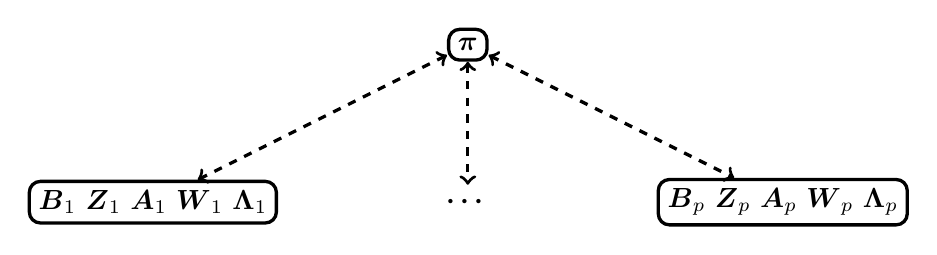
\begin{tikzpicture}
\tikzstyle{every path}=[very thick];
\path (0, 2) node (pi)[rounded corners, draw] {$\bs{\pi}$}
(-4, 0) node (node1)[rounded corners, draw] {$\bs{B}_1$ $\bs{Z}_1$ $\bs{A}_1$ $\bs{W}_1$ $\bs{\Lambda}_1$}
(0, 0) node (zero) {$\bs{\cdots}$}
(4, 0) node (nodep)[rounded corners, draw] {$\bs{B}_p$ $\bs{Z}_p$ $\bs{A}_p$ $\bs{W}_p$ $\bs{\Lambda}_p$};
\draw[dashed, <->] (pi) -- (node1);
\draw[dashed, <->] (pi) -- (zero);
\draw[dashed, <->] (pi) -- (nodep);
\end{tikzpicture}
\end{center}

\bibliography{vem_bib.bib}

\end{document}